\documentclass[a4paper,11pt,twoside]{report}
% THIS FILE SHOULD BE COMPILED BY pdfLaTeX

% ----------------------   PREAMBLE PART ------------------------------

% ------------------------ ENCODING & LANGUAGES ----------------------

\usepackage[utf8]{inputenc}
%\usepackage[MeX]{polski} % Not needed unless You have a name with polish symbols or sth
\usepackage[T1]{fontenc}
\usepackage[english, polish]{babel}


\usepackage{amsmath, amsfonts, amsthm, latexsym} % MOSTLY MATHEMATICAL SYMBOLS

\usepackage[final]{pdfpages} % INPUTING TITLE PDF PAGE - GENERATE IT FIRST!
%\usepackage[backend=bibtex, style=verbose-trad2]{biblatex}


\usepackage{commath} % various commands which can make writing math expressions easier --- documentation available at: https://ctan.gust.org.pl/tex-archive/macros/latex/contrib/commath/commath.pdf

\usepackage[hidelinks]{hyperref} % for hyperlinks, for example, urls, references to equations, entries in a bibliography --- hidelinks option removes rectangles around hiperlinks


% ---------------- MARGINS, INDENTATION, LINESPREAD ------------------

\usepackage[inner=20mm, outer=20mm, bindingoffset=10mm, top=25mm, bottom=25mm]{geometry} % MARGINS


\linespread{1.5}
\allowdisplaybreaks         % ALLOWS BREAKING PAGE IN MATH MODE

\usepackage{indentfirst}    % IT MAKES THE FIRST PARAGRAPH INDENTED; NOT NEEDED
\setlength{\parindent}{5mm} % WIDTH OF AN INDENTATION


%---------------- RUNNING HEAD - CHAPTER NAMES, PAGE NUMBERS ETC. -------------------

\usepackage{fancyhdr}
\pagestyle{fancy}
\fancyhf{}
% PAGINATION: LEFT ALIGNMENT ON EVEN PAGES, RIGHT ALIGNMENT ON ODD PAGES 
\fancyfoot[LE,RO]{\thepage} 
% RIGHT HEADER: zawartość \rightmark do lewego, wewnętrznego (marginesu) 
\fancyhead[LO]{\sc \nouppercase{\rightmark}}
% lewa pagina: zawartość \leftmark do prawego, wewnętrznego (marginesu) 
\fancyhead[RE]{\sc \leftmark}

\renewcommand{\chaptermark}[1]{\markboth{\thechapter.\ #1}{}}

% HEAD RULE - IT'S A LINE WHICH SEPARATES HEADER AND FOOTER FROM CONTENT
\renewcommand{\headrulewidth}{0 pt} % 0 MEANS NO RULE, 0.5 MEANS FINE RULE, THE BIGGER VALUE THE THICKER RULE


\fancypagestyle{plain}{
  \fancyhf{}
  \fancyfoot[LE,RO]{\thepage}
  
  \renewcommand{\headrulewidth}{0pt}
  \renewcommand{\footrulewidth}{0.0pt}
}



% --------------------------- CHAPTER HEADERS ---------------------

\usepackage{titlesec}
\titleformat{\chapter}
  {\normalfont\Large \bfseries}
  {\thechapter.}{1ex}{\Large}

\titleformat{\section}
  {\normalfont\large\bfseries}
  {\thesection.}{1ex}{}
\titlespacing{\section}{0pt}{30pt}{20pt} 

    
\titleformat{\subsection}
  {\normalfont \bfseries}
  {\thesubsection.}{1ex}{}


% ----------------------- TABLE OF CONTENTS SETUP ---------------------------

\def\cleardoublepage{\clearpage\if@twoside
\ifodd\c@page\else\hbox{}\thispagestyle{empty}\newpage
\if@twocolumn\hbox{}\newpage\fi\fi\fi}


% THIS MAKES DOTS IN TOC FOR CHAPTERS
\usepackage{etoolbox}
\makeatletter
\patchcmd{\l@chapter}
  {\hfil}
  {\leaders\hbox{\normalfont$\m@th\mkern \@dotsep mu\hbox{.}\mkern \@dotsep mu$}\hfill}
  {}{}
\makeatother

\usepackage{titletoc}
\makeatletter
\titlecontents{chapter}% <section-type>
  [0pt]% <left>
  {}% <above-code>
  {\bfseries \thecontentslabel.\quad}% <numbered-entry-format>
  {\bfseries}% <numberless-entry-format>
  {\bfseries\leaders\hbox{\normalfont$\m@th\mkern \@dotsep mu\hbox{.}\mkern \@dotsep mu$}\hfill\contentspage}% <filler-page-format>

\titlecontents{section}
  [1em]
  {}
  {\thecontentslabel.\quad}
  {}
  {\leaders\hbox{\normalfont$\m@th\mkern \@dotsep mu\hbox{.}\mkern \@dotsep mu$}\hfill\contentspage}

\titlecontents{subsection}
  [2em]
  {}
  {\thecontentslabel.\quad}
  {}
  {\leaders\hbox{\normalfont$\m@th\mkern \@dotsep mu\hbox{.}\mkern \@dotsep mu$}\hfill\contentspage}
\makeatother



% ---------------------- TABLES AD FIGURES NUMBERING ----------------------

\renewcommand*{\thetable}{\arabic{chapter}.\arabic{table}}
\renewcommand*{\thefigure}{\arabic{chapter}.\arabic{figure}}


% ------------- DEFINING ENVIRONMENTS FOR THEOREMS, DEFINITIONS ETC. ---------------

\makeatletter
\newtheoremstyle{definition}
{3ex}%                           % Space above
{3ex}%                           % Space below
{\upshape}%                      % Body font
{}%                              % Indent amount
{\bfseries}%                     % Theorem head font
{.}%                             % Punctuation after theorem head
{.5em}%                          % Space after theorem head, ' ', or \newline
{\thmname{#1}\thmnumber{ #2}\thmnote{ (#3)}}
\makeatother

\theoremstyle{definition}
\newtheorem{theorem}{Theorem}[chapter]
\newtheorem{lemma}[theorem]{Lemma}
\newtheorem{example}[theorem]{Example}
\newtheorem{proposition}[theorem]{Proposition}
\newtheorem{corollary}[theorem]{Corollary}
\newtheorem{definition}[theorem]{Definition}
\newtheorem{remark}[theorem]{Remark}

% --------------------- END OF PREAMBLE PART (MOSTLY) --------------------------





% -------------------------- USER SETTINGS ---------------------------

\newcommand{\tytul}{Zastosowanie techniki transfer learning wzadaniuklasyfikacjiszeregów czasowych}
\renewcommand{\title}{Transfer learning for time series classification}
\newcommand{\type}{Master} % Master OR Engineer
\newcommand{\supervisor}{Agnieszka Jastrzębska, PhD} % TITLE AND NAME OF THE SUPERVISOR

%---------------------------Moje ustawienia-----------------------------

\DeclareMathOperator{\real}{\mathbb{R}}
\DeclareMathOperator{\natur}{\mathbb{N}}

\begin{document}
\sloppy
\selectlanguage{english}

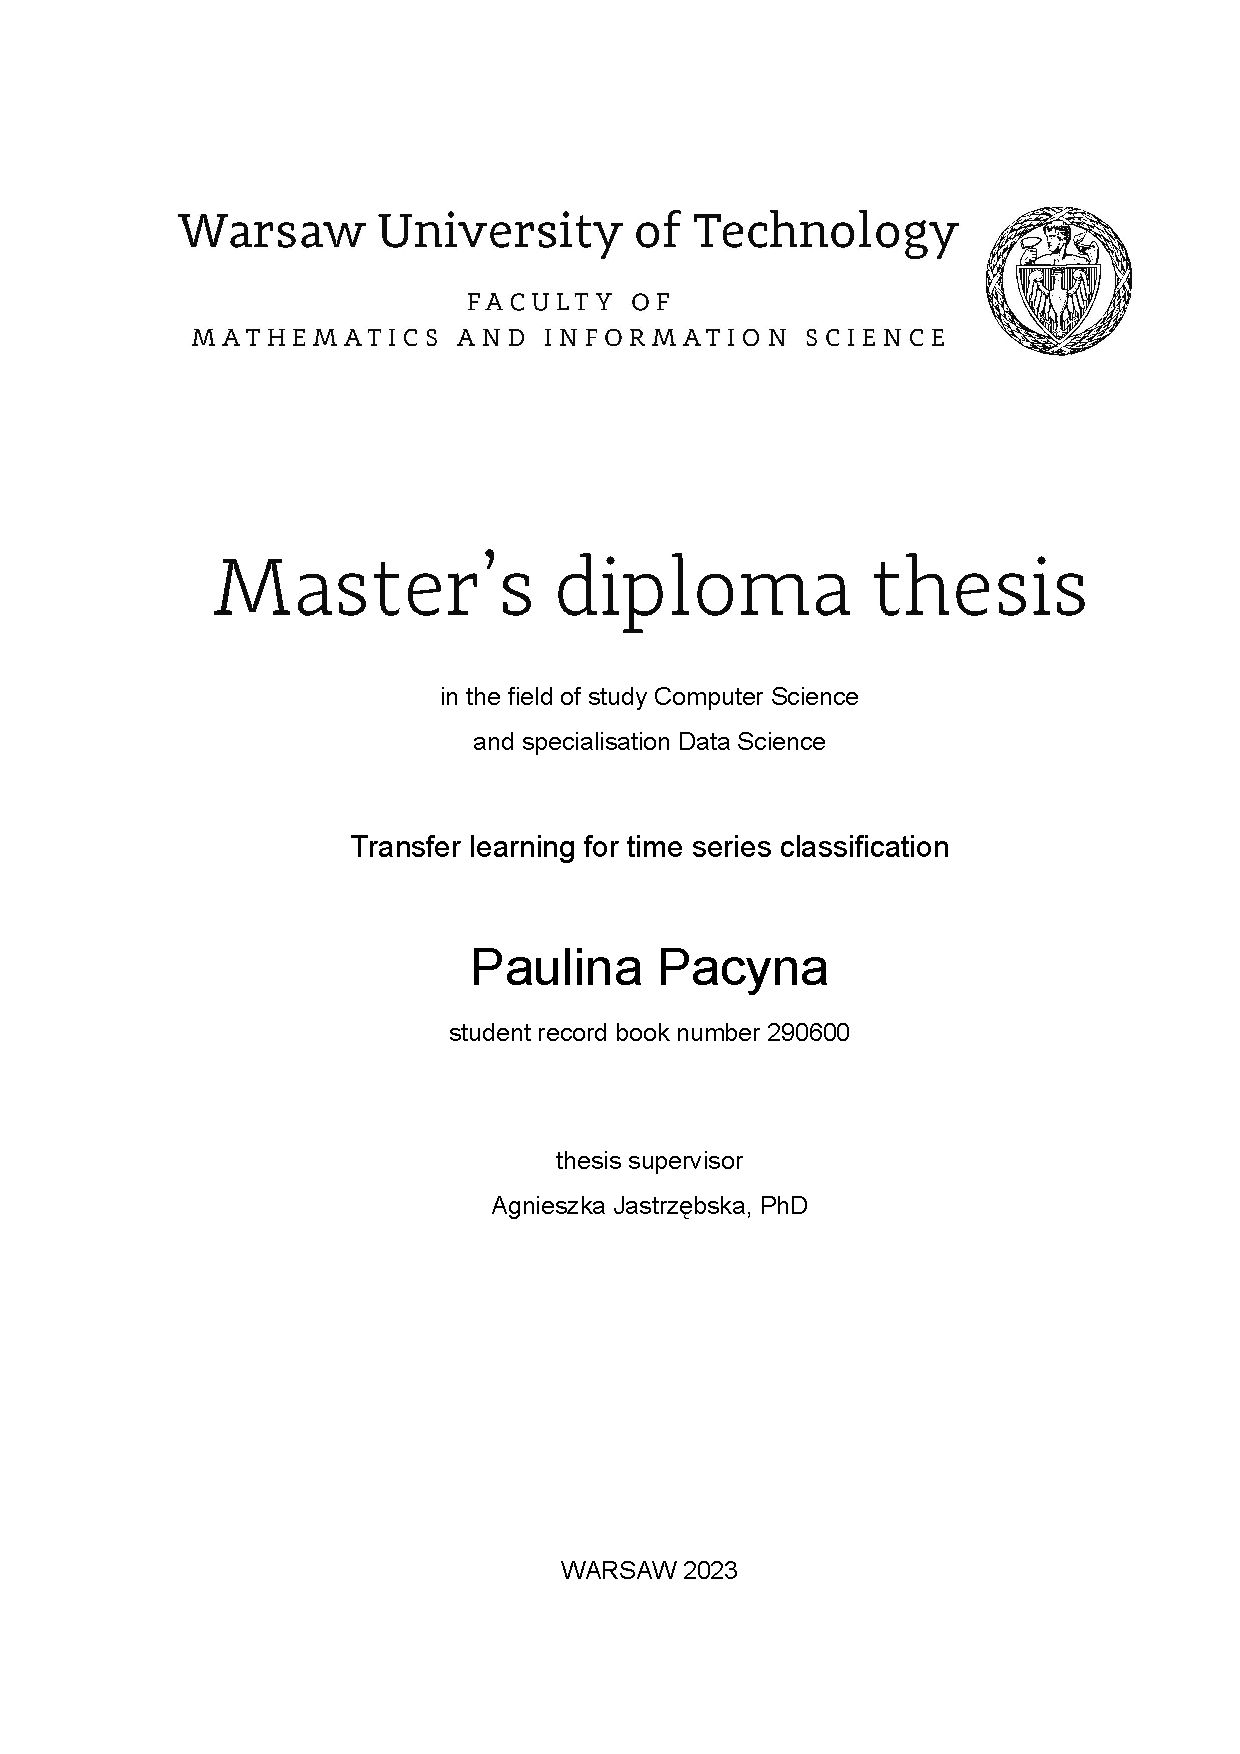
\includepdf[pages=-]{titlepage-en} % THIS INPUTS THE TITLE PAGE

\null\thispagestyle{empty}\newpage

% ------------------ PAGE WITH SIGNATURES --------------------------------

%\thispagestyle{empty}\newpage
%\null
%
%\vfill
%
%\begin{center}
%\begin{tabular}[t]{ccc}
%............................................. & \hspace*{100pt} & .............................................\\
%supervisor's signature & \hspace*{100pt} & author's signature
%\end{tabular}
%\end{center}
%


% ---------------------------- ABSTRACTS -----------------------------

{  \fontsize{12}{14} \selectfont
\begin{abstract}

\begin{center}
\title
\end{center}
Loremmmm ipsum dolor sit amet, consetetur sadipscing elitr, sed diam nonumyeirmod tempor invidunt ut labore et dolore magna aliquyam erat, sed diamvoluptua. At vero eos et accusam et justo duo dolores et ea rebum. Stet clita kasd gubergren, no sea takimata sanctus est Lorem ipsum dolor sit amet.

Lorem ipsum dolor sit amet, consetetur sadipscing elitr, sed diam nonumyeirmod tempor invidunt ut labore et dolore magna aliquyam erat, sed diamvoluptua. At vero eos et accusam et justo duo dolores et ea rebum. Stet clita kasd gubergren, no sea takimata sanctus est Lorem ipsum dolor sit amet.\\

\noindent \textbf{Keywords:} keyword1, keyword2, ...
\end{abstract}
}

\null\thispagestyle{empty}\newpage


{\selectlanguage{polish} \fontsize{12}{14}\selectfont
\begin{abstract}

\begin{center}
\tytul
\end{center}

Lorem ipsum dolor sit amet, consetetur sadipscing elitr, sed diam nonumyeirmod tempor invidunt ut labore et dolore magna aliquyam erat, sed diamvoluptua. At vero eos et accusam et justo duo dolores et ea rebum. Stet clita kasd gubergren, no sea takimata sanctus est Lorem ipsum dolor sit amet.

Lorem ipsum dolor sit amet, consetetur sadipscing elitr, sed diam nonumyeirmod tempor invidunt ut labore et dolore magna aliquyam erat, sed diamvoluptua. At vero eos et accusam et justo duo dolores et ea rebum. Stet clita kasd gubergren, no sea takimata sanctus est Lorem ipsum dolor sit amet.\\

\noindent \textbf{Słowa kluczowe:} slowo1, slowo2, ...
\end{abstract}
}


%% --------------------------- DECLARATIONS ------------------------------------
%
%%
%%	IT IS NECESSARY OT ATTACH FILLED-OUT AUTORSHIP DEECLRATION. SCAN (IN PDF FORMAT) NEEDS TO BE PLACED IN scans FOLDER AND IT SHOULD BE CALLED, FOR EXAMPLE, DECLARATION_OF_AUTORSHIP.PDF. IF THE FILENAME OR FILEPATH IS DIFFERENT, THE FILEPATH IN THE NEXT COMMAND HAS TO BE ADJUSTED ACCORDINGLY.
%%
%%	command attacging the declarations of autorship
%%
%\includepdf[pages=-]{scans/declaration-of-autorship}
%\null\thispagestyle{empty}\newpage
%
%% optional declaration
%%
%%	command attaching the declaataration on granting a license
%%
%\includepdf[pages=-]{scans/declaration-on-granting-a-license}
%%
%%	.tex corresponding to the above PDF files are present in the 3. declarations folder 
%
\null\thispagestyle{empty}\newpage
% ------------------- TABLE OF CONTENTS ---------------------
% \selectlanguage{english} - for English
\pagenumbering{gobble}
\tableofcontents
\thispagestyle{empty}
\newpage % IF YOU HAVE EVEN QUANTITY OD PAGES OF TOC, THEN REMOVE IT OR ADD \null\newpage FOR DOUBLE BLANK PAGE BEFORE INTRODUCTION


% -------------------- THE BODY OF THE THESIS --------------------------------

\null\thispagestyle{empty}\newpage
\pagestyle{fancy}
\pagenumbering{arabic}
\setcounter{page}{11}


\chapter*{Introduction}
\markboth{}{Introduction}
\addcontentsline{toc}{chapter}{Introduction}

What is the thesis about? What is the content of it? What is the Author's contribution to it?
\par
WARNING!  In a diploma thesis which is a team project: Description of the work division in the team, including the scope of each co-author’s contribution to the practical part (Team Programming Project) and the descriptive part of the diploma thesis. 
\par
\chapter{Related works}
In this chapter, we describe several algorithms used in time series classification. We will also recall theoretical definitions and distinctions used to describe transfer learning. 
\section{Time series classification}
Time series is an ordered collection of observations indexed by time. 
$$X = (x_t)_{t\in T} = (x_1, ... , x_T),\ x_t\in \real$$
The time index $T$ can represent any collection with the natural order. It can relate to a point in time when the measurement was observed or represent a point in space measured along the X-axis. We assume that indices are spaced evenly in the set $T$. The realization or observation $x_t$ in the times series is a numerical value describing the phenomena we observe, for example, the amplitude of a sound, stock price, or y-coordinate. Time series classification is a problem of finding the optimal mapping between a set of time series and corresponding classes.

%Time series classification can be formulated as follows:
%Given a dataset  $D = {(X_i, y_i)}_{i=1}^N$, where $X_i \in 2^\real$ is a time series and $y_i\in {1, ..., N} = C$, we would like to find a function (called classifier) $f_\theta :2^\real \leftarrow C$ such that 
%$$f_\theta (X_i) = y_i$$. 

\subsection{Dynamic Time Warping with k-Nearest Neighbour}
The Dynamic Time Warping \cite{bake_off} with k-Nearest Neighbour classifier uses a distance-based algorithm with a specific distance measure. A DWT distance between time series $X^1$, $X^2$ of equal lengths is:
$$DTW(X^1, X^2) = \min\{ \sum_{i=1}^S dist(x^1_{e_i}, x^2_{f_i}):(e_i)_{i=1}^S, (f_i)_{i=1}^S\in 2^T\}$$
subject to:
\begin{itemize}
\item $e_1 = 1, f_1 = 1, e_S= N, f_S = N$
\item $|e_{i+1} - e_i | \leq 1$, $|f_{i+1} - f_i | \leq 1$
\end{itemize}
The measure defined above, used in the k-Nearest Neighbour classifier, is often used as a benchmark classifier. 
\subsection{Multi Layer Perceptron}
The Multi Layer Perceptron (MLP) is the first artificial neural network architecture proposed in \cite{dl_tsc} and can be used for time series classification task. 
%A MLP network can be formally defined as a function depending on a set \textit{weights} $\theta_i$. 
%$$MLP(X; \theta_1,\dots , \theta_M, \beta_1,\dots , \beta_M) = f_M( \beta_M +  \theta_M \cdot (f_{M-1}( \beta_{M-1} +  \theta_{M-1} \cdot (\dots f_1( \beta_1 +  \theta_1 \cdot X)))))$$
Formally, the MLP network can be defined as a composition of $layer$ functions. The network returns a vector that usually represents the probability distribution over the set of classes.
$$MLP(X; \theta_1,\dots , \theta_M, \beta_1,\dots , \beta_M) = L_M(\dots L_2(L_1(X;\theta_1, \beta_1);\theta_2, \beta_2);\theta_M, \beta_M)$$
Each layer $L_i: \real^M \rightarrow \real^N$ is a function that depends on the parameters $\theta \in r^{M\times N}, \beta in \real^N$
$$L_i(X, ; \theta_i, \beta_i) = f_i(X \theta_i  + \beta_i)$$
Function $f_i: \real^N \rightarrow \real^N$ is an arbitrary chosen non-linear function. The number of layers and dimension of weights in hidden layers is also arbitrary. The weights in first and last layer have to match the dimensionality of input data (e.g. the length of time series) and number of classes. The output of the last layer is interpreted as a probability distribution over the set of classes. 

The disadvantage of using Multi Layer Perceptrons for time series classification is that the input size is fixed. All time series is the training data must have the same length. In transfer learning, this means that if we want to reuse the source network (or a set of first layers from the network), the target dataset must consists of time series of the same length. 

The MLP architecture fails at understanding the temporal dependencies \cite{dl_tsc}. Each input values in the time series is treated separately, because it is multiplied by a separate row in the weight matrix. 

\subsection{Convolutional Neural Networks}
Convolutional Neural Networks are widely used in image recognition. A convolution applied for a time series can be interpreted as sliding a filter over the time series. A convolutional layer is a set of functions called convolutions or filters. The filter is applied at a given point, taking into account values that surrounds the point. 

To define the convolution operation, let's assume the input is a matrix $X \in \real^{(N_1, \dots, N_K)}$. In case of images, number of dimensions $K$ is often equal to $3$ (height, width, channels), for univariate time series we can assume just one dimension, and for multivariate time series wee need two dimensions - (feature, time). 
The filter consist of a matrix of weights $M \in \real^{(P_1, \dots, P_K)}$. 
Usually, $P_l$ are odd numbers, so that we can index the matrix with symmetrical numbers: $ (\frac{-P_l+1}{2},  \frac{-P_l+3}{2}, \dots, 0, \dots, \frac{P_l-1}{2})$. The $0$ index marks the center of the matrix. 
%TODO - powolac sie czemu nieparzyscie

Finally the convolution $*$ is defined as follows:
$$(X*M)_{i_1, \dots, i_K} = \sum_{l_1=\frac{-P_1+1}{2}}^{\frac{P_1-1}{2}} \cdots \sum_{l_K=\frac{-P_K+1}{2}}^{\frac{P_K-1}{2}} M_{l_1, \dots, l_K} X_{i_1 + l_1, \dots, i_K + l_K}$$

The result of the convolution is passed elementwise to a nonlinear function. The nonlinear function together with the convolution operation will be called a filter.

In case of univariate time series the first layer of convolutional neural network is one-dimensional. The output of the first layer has dimensions (length of time series - the length of the filter - 1, number of filters). Below we define the value of the output for filter $i$  
$$ y_{t, i} = f_i([\theta_{\frac{-M+1}{2}}^i, \dots , \theta_{\frac{M-1}{2}}^i] \cdot [X_{t_+\frac{-M+1}{2}}, \dots, X_{t+\frac{M-1}{2}}]),$$ 
where $\cdot$ is a dot product
The weights $\theta^i$ are different for each filter.
The same filter is applied over the whole length of time series. This is called \textit{weight sharing} and it enables the patterns regardless of the position in the time series. 

The architecture of the convolutional layer is not dependent of the size of the input data. Regardless the size of input data, number of filters and size of filters remain the same, only the output sizes depends on the input size. Therefore, if the convolutional layer is  succeeded by layers with the same property, like other convolutional layers or Global Pooling with Dense Layer (see section \ref{FCN}), the whole network may be invariant to the input sizes \cite{dl_tsc}. Such networks may be interesting in terms of transfer learning, as the sizes of time series in the source task and in the target task do not have to match.  

\subsection{Fully Convolutional Networks}\label{FCN}
Fully Convolutional Networks are convolutional networks used in time series classification. A sample architecture of a Fully Convolutional Network proposed is in \cite{dl_tsc}. The first layers in the network are 3 blocks of convolutional layers with ReLU activation function followed by batch normalisation layers. The output of the last block is passed to a global pooling layer. The global pooling layer averages the output through the time axis, resulting in a vector of length equal to the number of feature maps in the last convolutional layer. The averaged vector is passed to a block of 2 fully connected layers. Figure \ref{FCN_img} shows a visualisation of the network.\\

\begin{figure}[!ht]
\centering
\includegraphics[width=13cm]{imgs/FCN.png}
\label{FCN_img}
\caption{Architecture of a Fully Convolutional Network. Source: \cite{dl_tsc}}
\end{figure}




Because the architecture of convolutional layers does not depend on the size of input data and the convolutional layer are followed by pooling over the time axis, the whole networks is capable of processing data of variable lengths.


\section{Transfer learning}
Transfer learning is a technique that attempts to apply knowledge learned  while solving one task to enhance the learning process for another task. Formally, the problem can be described using the notions of tasks and domains \cite{survey_transfer_learning, comp_survey_transfer_leaerning}. A \textit{Domain} is a pair $\mathcal{D}=(\mathcal{X}, P(\mathcal{X}))$, where $\mathcal{X}$ is the feature space (e.g. the time series observations, and $P(\mathcal{X})$ is the probability distribution over the feature space. A \textit{Task} is a pair of label space $\mathcal{Y}$ and the decision function $f$, $\mathcal{T} = (\mathcal{Y}, f)$. The decision function $f$ is learned from $\mathcal{X}, P(\mathcal{X}), \mathcal{Y}$ in the learning process.

Transfer learning attempts to utilize knowledge  domain/domains and task/tasks. Formally, given $S \in \natur$ source domains and source tasks ($\{(\mathcal{D}_i^S,\mathcal{T}_i^S: \i=1, \dots, S \}$) and $T \in \natur$ target domains and target tasks ($\{(\mathcal{D}_i^T,\mathcal{T}_i^T: \i=1, \dots, S \}$) transfer learning utilizes knowledge learned from source domains and tasks to improve the learning process of decision functions in target tasks $\mathcal{T}_i^T$
\subsection{Types of transfer learning}

\subsection{Characteristics of a good source domain}

In the field of image processing, it is very common to use convolutional neural networks \mbox{pre-trained} with the ImageNet dataset \cite{imagnet}.  ImageNet is a large dataset of human-annotated images. It contains 1 milion labeled images of 1000 classes. The label space consists of fine grained classes such as breeds of dogs and cats, but also coarse-grained classes like \textit{red wine} and \textit{traffic light}. As transfer learning based on this dataset became more popular and successful, a question arisen: Which features of this dataset makes it so good for this task?.

A study conducted in \cite{imagnet} attempts to answer this question. The first hypothesis is that the volume of the dataset is relevant to train accurate, general classfiers. The authors compared models pretrained on the original dataset and models based on sampled subsets (reduced 2, 4 8 and 20 times).The results shown that the more training examples, the better results. The accuracy of the initial classifier occured to be more dependent on the size of dataset than the accuracy of classifiers fine-tuned from the former classifier.

Next experiments answer considerations on the label space. The authors examine if the granularity of the label space is essential for the problem. To compare the results, the label space is clustered and 127 classes are derived from the initial 1000 classes. Pre-training with the reduced label space has a minimal negative impact on accuracy of classifiers fine-tuned from this classifier. This suggest that such a fine division may not be needed.

Finally, the last question is if we train the classfier on the reduced label space with 127 classes, will it be able to distinguish between the fine-grained classes. To examine that, the authors extracted features from the first layers of the networks trained on recuded label space. Then, the authors performed classfication with 1-NN and 5-NN models on the extracted feature space, but with 1000 classes. The fidings are that the k-NN classifier performs $15\%$ worse on reduced dataset vs normal dataset. This shows that CNNs are capable of implicitly learning representative features distinctive beetween similar classes even when trained on coarse-grained classes.     

While the article \cite{imagnet} does not conclude which single feature of ImageNet dataset makes it so efficient as a source dataset for transfer learning, it is clear that all properties of this dataset are important for the accuracy of the t. 
% ------------------------------- BIBLIOGRAPHY ---------------------------
% LEXICOGRAPHICAL ORDER BY AUTHORS' LAST NAMES
% FOR AMBITIOUS ONES - USE BIBTEX


\bibliographystyle{plain} % We choose the "plain" reference style
\bibliography{refs} % Entries are in the refs.bib file


\pagenumbering{gobble}
\thispagestyle{empty}



% ----------------------- LIST OF SYMBOLS AND ABBREVIATIONS ------------------
%\chapter*{List of symbols and abbreviations}
%
%\begin{tabular}{cl}
%nzw. & nadzwyczajny \\
%* & star operator \\
%$\widetilde{}$ & tilde 
%\end{tabular}
%\\
%If you don't need it, delete it.
%\thispagestyle{empty}
%
%
%% ----------------------------  LIST OF FIGURES --------------------------------
%\listoffigures
%\thispagestyle{empty}
%If you don't need it, delete it.
%
%
%% -----------------------------  LIST OF TABLES --------------------------------
%\renewcommand{\listtablename}{Spis tabel}
%\listoftables
%\thispagestyle{empty}
%If you don't need it, delete it.
%
%% -----------------------------  LIST OF APPENDICES ---------------------------
%\chapter*{List of appendices}
%\begin{enumerate}
%\item Appendix 1
%\item Appendix 2
%\item In case of no appendices, delete this part.
%\end{enumerate}
%\thispagestyle{empty}


\end{document}
